%*********************************************************
\section{Bayesian Calibration}\label{sec:bc_modular_bayes}
%*********************************************************

% Introductory paragraph
In a simulation of a physical system, complementary to the observed (measured) data and simulator prediction, it is also assumed here that there exists true process, true response, and true model parameters. 
The relationships among these elements are illustrated in Fig.~\ref{fig:ch5_hm_error_model}.
The goal of model calibration is, broadly speaking, to learn the true (but unknown) model parameters such that the agreement between simulator prediction and observed data is improved.
In practice, however, observed data on the true response are finite and often imprecise.
Moreover, the computer simulator that simulates the true underlying process is an approximation that might contain an unknown systematic bias.
All of these constitute sources of uncertainty in the estimation (i.e., calibration) of the model parameters based on experimental data.
A more robust calibration procedure requires accounting for the aforementioned sources of uncertainty.
Bayesian framework provides a consistent approach for such calibration while simultaneously taking into account multiple sources of uncertainty.
\begin{figure}[bth]	
	\centering
	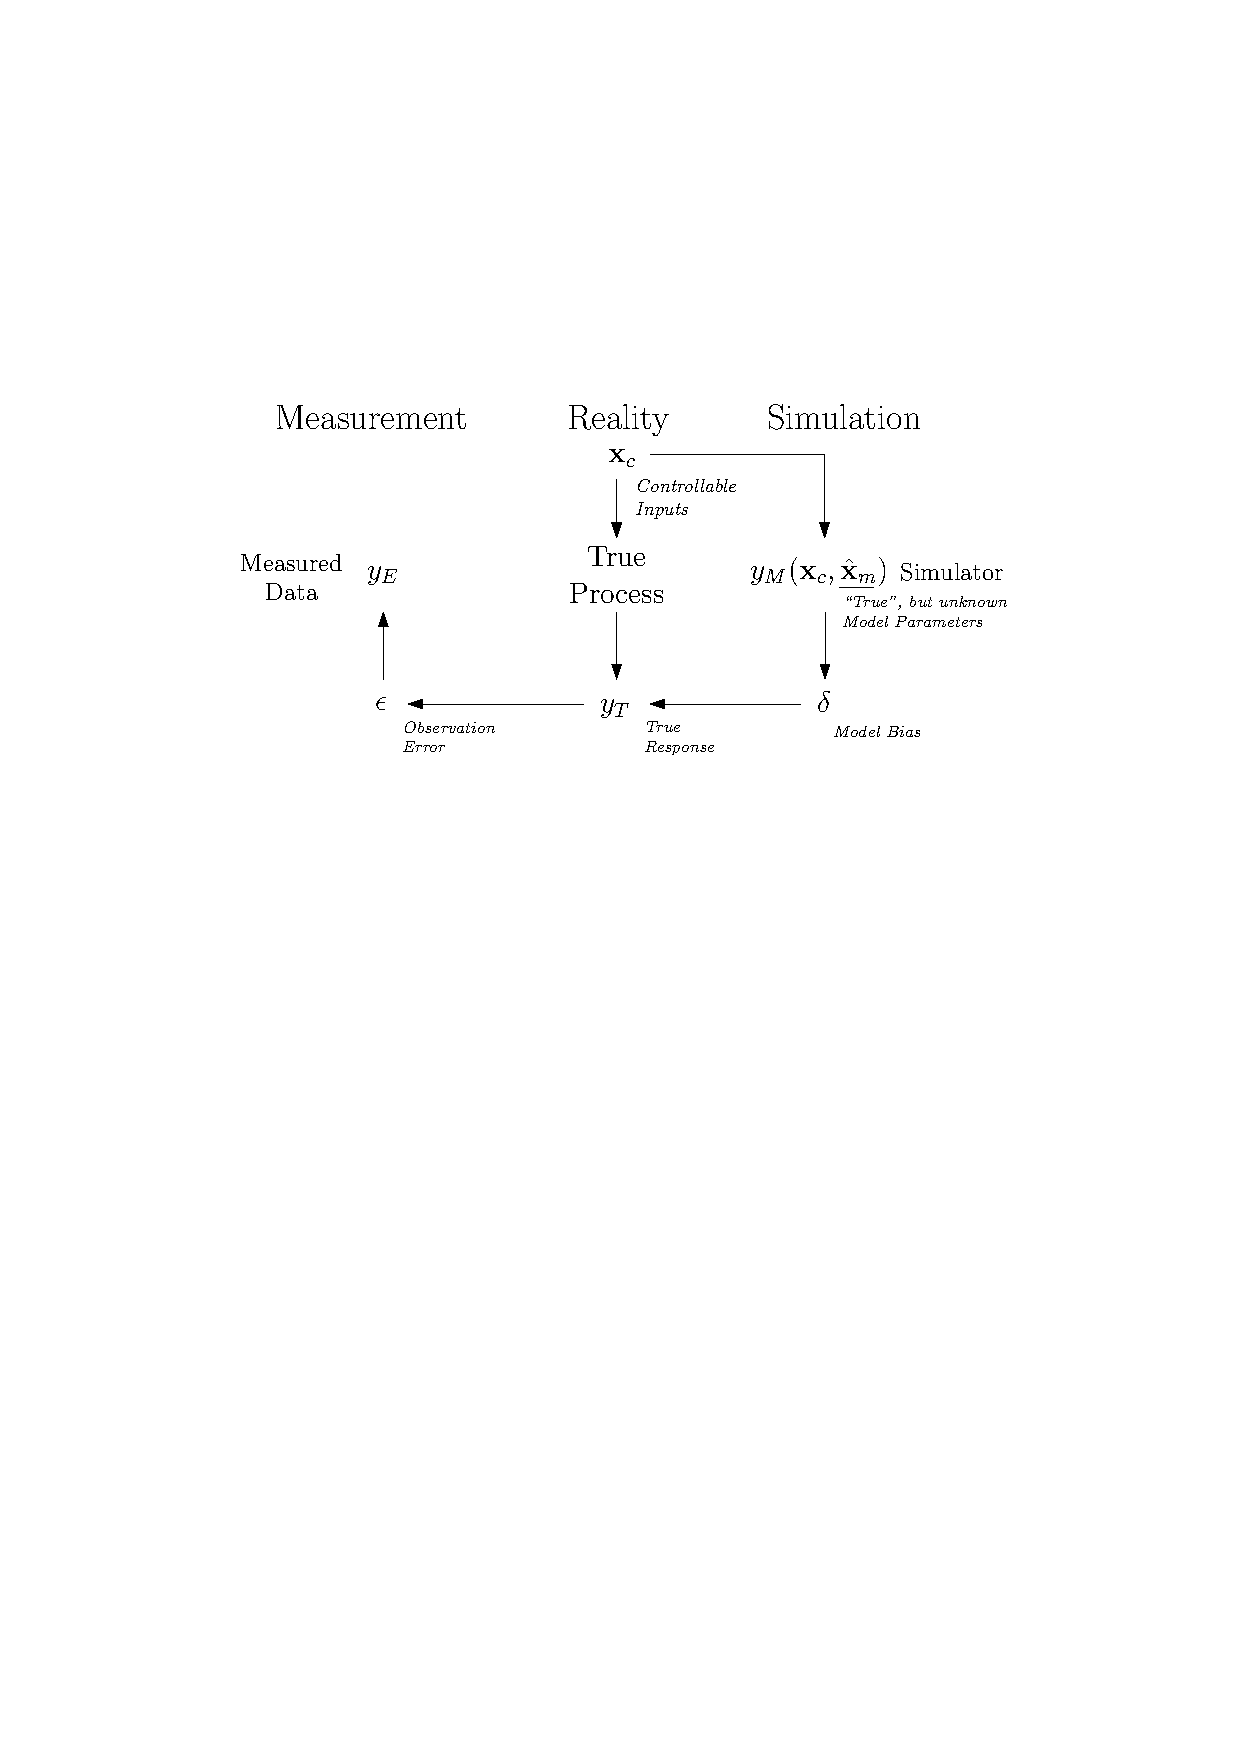
\includegraphics[width=1.0\textwidth]{../figures/chapter5/figures/HMErrorModel}
	\caption[Relationships between sources of uncertainty in a model calibration.]{Sources of uncertainty and their relationships in a model calibration (adapted from \cite{Huard2006}).}
	\label{fig:ch5_hm_error_model}
\end{figure}

% Bayesian framework
The relationships between these sources of uncertainties can be expressed additively as it was given in Eq.~(\ref{eq:bc_observation_true}).
The Bayesian framework for model calibration then begins by constructing a probabilistic model of $y_E$. 
That is, it aims at formulating the data generating process $\mathcal{Y}_E(\bm{x}_c;\lambda)$.
This model implies that the experimental data $y_E$ taken at particular $\bm{x}_c$ observed at $\lambda$ is a realization of a stochastic process.
Furthermore, this probabilistic modeling entails casting any \emph{uncertain} element in Eq.~(\ref{eq:bc_observation_true}) either as random variable or stochastic process.

% Likelihood
As such, 
\begin{equation}
    \begin{split}
        \mathcal{Y}_M & \equiv \mathcal{Y}_M (\bm{x}_c, \hat{\bm{x}}_m; \lambda) \thicksim  p(y_m | \bm{x}_c, \hat{\bm{x}}_m; \lambda) \\
        (\mathcal{Y}_T - \mathcal{Y}_M) & \equiv \mathcal{D}(\bm{x}_c; \lambda) \thicksim p(\delta | \psi_{\delta}, \bm{x}_c; \lambda) \\
        (\mathcal{Y}_E - \mathcal{Y}_T) & \equiv \mathcal{E}_y(\lambda) \thicksim p(\epsilon_y | \psi_{\epsilon_y}; \lambda) \\
    \end{split}
\label{eq:bc_additive_formulation}
\end{equation}

% Data Generating Process
Under the additive formulation, the data generating process for $\mathcal{Y}_E$ can be obtained by adding all the three terms above.
Assuming those three terms are independent, the \gls[hyper=false]{pdf} of $\mathcal{Y}_E$ is defined as the convolution of the terms,
\begin{equation}
  p(y_E) = (p(y_M | \bm{x}_c, \hat{\bm{x}}_m; \lambda) * p(\delta | \bm{x}_c, \psi_{\delta}; \lambda) * p(\epsilon_y | \psi_{\epsilon_y}; \lambda))(y_E)
\label{eq:bc_additive_convolution}
\end{equation}
where $*$ is the symbol for the convolution operation.

% The Likelihood
Given the experimental data $\mathbf{y}$ taken at $\mathbf{x}_c$ and observed at $\lambda$, the likelihood function is then defined as follows
\begin{equation}
  \mathcal{L}(\hat{\bm{x}}_m, \psi_\delta, \psi_{\epsilon_y}; \mathbf{y}, \mathbf{x}_c, \lambda) \equiv p(y_E = \mathbf{y} | \bm{x}_c = \mathbf{x}_c, \hat{\bm{x}}_m, \psi_\delta, \psi_{\epsilon_y} ; \lambda)
\label{eq:bc_likelihood}
\end{equation}
For conciseness, 
it is always implicitly assumed in the following that a likelihood function is always defined for given data and controllable inputs such that the notation $\mathcal{L}(\hat{\bm{x}}_m, \psi_\delta, \psi_{\epsilon_y}; \lambda)$ is sufficient.

% Full probability model
Following Bayes' theorem, the probability of the model parameters $\bm{x}_m$
\begin{equation}
  p(\hat{\bm{x}}_m, \psi_\delta, \psi_{\epsilon_y} | \mathbf{y}, \mathbf{x}_c; \lambda) = \frac{\mathcal{L}(\hat{\bm{x}}_m, \psi_\delta, \psi_{\epsilon_y} ; \mathbf{y}, \mathbf{x}_c, \lambda) \cdot p(\hat{\bm{x}}_m) \cdot p(\psi_{\epsilon_y}; \lambda) \cdot p(\psi_{\delta}; \lambda)}{p(y_E = \mathbf{y} | \bm{x}_c = \mathbf{x}_c ; \lambda)}
\label{eq:bc_}
\end{equation}
where the denominator is defined as,
\begin{equation}
	p(y_E = \mathbf{y} | \bm{x}_c = \mathbf{x}_c ; \lambda) = \int \mathcal{L}(\hat{\bm{x}}_m, \psi_\delta, \psi_{\epsilon_y}; \mathbf{y}, \mathbf{x}_c, \lambda) \cdot p(\hat{\bm{x}}_m) \cdot p(\psi_{\epsilon_y}) \cdot p(\psi_{\delta}) d\psi_{\epsilon_y} d\psi_\delta
\label{eq:}
\end{equation}
